% Session 08 – Deep Networks History & Vanishing Gradients
% Course: Deep Learning (AI Systems Lab)
% Instructors: Prof. S R M Prasanna & Dr. Sunil Saumya
% Generated from: session08_transcript.vtt + session08_visual_extraction.md

\documentclass[12pt,a4paper]{article}
\usepackage{amsmath,amsthm,amssymb,mathtools}
\usepackage{tikz}
\usetikzlibrary{arrows.meta,positioning,shapes.geometric,calc,fit,backgrounds}
\usepackage{graphicx}
\usepackage{booktabs,tabularx,multirow}
\usepackage[ruled,vlined,linesnumbered]{algorithm2e}
\usepackage[most]{tcolorbox}
\usepackage{hyperref}
\usepackage[capitalize,noabbrev]{cleveref}
\usepackage[margin=1in]{geometry}
\usepackage{fancyhdr}
\usepackage{enumitem}
\usepackage{xcolor}

% -------------------------------------------------------
% tcolorbox environments
% -------------------------------------------------------
\newtcolorbox{keyinsight}[1][]{colback=blue!5!white,colframe=blue!75!black,fonttitle=\bfseries,title=Key Insight,#1}
\newtcolorbox{example}[1][]{colback=green!5!white,colframe=green!75!black,fonttitle=\bfseries,title=Example,#1}
\newtcolorbox{warningbox}[1][]{colback=red!5!white,colframe=red!75!black,fonttitle=\bfseries,title=Warning,#1}

% -------------------------------------------------------
% amsthm environments
% -------------------------------------------------------
\newtheorem{theorem}{Theorem}[section]
\newtheorem{lemma}[theorem]{Lemma}
\newtheorem{definition}{Definition}[section]
\newtheorem{remark}{Remark}[section]

% -------------------------------------------------------
% Page style
% -------------------------------------------------------
\pagestyle{fancy}
\fancyhf{}
\rhead{Session 08 -- Deep Learning}
\lhead{AI Systems Lab}
\cfoot{\thepage}
\renewcommand{\headrulewidth}{0.4pt}

\hypersetup{
  colorlinks=true,
  linkcolor=blue!60!black,
  urlcolor=blue!60!black,
  pdftitle={Session 08 -- Deep Networks History and Vanishing Gradients},
}

% -------------------------------------------------------
% Convenience macros
% -------------------------------------------------------
\newcommand{\sigmoid}{\sigma}
\newcommand{\relu}{\mathrm{ReLU}}
\newcommand{\Loss}{\mathcal{L}}

% -------------------------------------------------------
\begin{document}
% -------------------------------------------------------

% ===========================================================
% TITLE PAGE
% ===========================================================
\begin{titlepage}
  \centering
  \vspace*{2cm}
  {\Large\bfseries AI Systems Lab -- Deep Learning Course\par}
  \vspace{0.5cm}
  \rule{\linewidth}{1pt}
  \vspace{0.5cm}

  {\LARGE\bfseries Session 08\par}
  \vspace{0.3cm}
  {\large\itshape Transition to Deep Networks: History, Vanishing \&
   Exploding Gradients, and Solutions\par}

  \vspace{0.5cm}
  \rule{\linewidth}{1pt}
  \vspace{1cm}

  \begin{tabular}{ll}
    \textbf{Video}       & \url{https://vimeo.com/1146137830} \\[4pt]
    \textbf{Slide Deck}  & \texttt{04-PyTorchDL-Autograd} \\[4pt]
    \textbf{Duration}    & $\approx$ 1 hour 22 minutes \\[4pt]
    \textbf{Instructors} & Prof.\ S R M Prasanna \&\ Dr.\ Sunil Saumya \\[4pt]
    \textbf{Institution} & IIIT Dharwad \\[4pt]
    \textbf{Date}        & 2024 \\
  \end{tabular}

  \vspace{1.5cm}

  \begin{abstract}
    \noindent
    Session~8 marks the pivotal transition from shallow artificial neural
    networks (ANNs) to deep networks.  The lecture opens by recapping the
    historical arc from the single-layer perceptron through the
    multi-layer perceptron (MLP) and backpropagation, then explains the
    six converging factors that enabled the modern deep learning
    resurgence after the ``AI winter'' of the late 1990s.  The central
    topic is the \emph{vanishing/exploding gradient problem} (VGP/EGP):
    why sigmoid activations cause gradients to shrink exponentially as
    they propagate backwards through many layers, stalling learning in
    early layers.  A concrete four-layer numerical walkthrough
    demonstrates the phenomenon.  The session concludes with a
    three-step solution framework: (1)~identify the gradient problem,
    (2)~explore weight initialisation (greedy layer-wise unsupervised
    pre-training), and (3)~replace sigmoid with the Rectified Linear
    Unit (ReLU), whose constant derivative of~1 eliminates gradient
    decay.
  \end{abstract}

  \vfill
  {\small Course notes compiled from lecture transcript and visual
  extractions.}
\end{titlepage}

% ===========================================================
% TABLE OF CONTENTS
% ===========================================================
\tableofcontents
\newpage

% ===========================================================
\section{Introduction}
\label{sec:introduction}
% ===========================================================

Sessions~1 through~7 of this course established the complete mechanics
of feed-forward neural networks: from the basic perceptron and
multi-layer perceptron (MLP) to the backpropagation learning algorithm
and its convergence properties.  At the close of that arc the natural
question arose: \emph{can we simply add more layers and neurons to
obtain a more powerful model?}

The answer turns out to be: \emph{yes, in principle -- but only after
overcoming a critical obstacle.}  Session~8 tells that story.  It
explains why deep networks were conceptualised as early as the 1990s
yet could not be trained in practice for nearly fifteen years, what the
root cause of the failure was, and what two complementary techniques
finally unlocked the deep learning revolution that began around 2006.

\begin{keyinsight}
The transition from shallow ANNs to deep networks was not driven by a
single algorithmic breakthrough.  It was the \emph{convergence} of six
enabling factors -- increased data, greater compute, and targeted
refinements to backpropagation -- that made deep learning practically
feasible.
\end{keyinsight}

The lecture is delivered jointly by \textbf{Prof.\ S R M Prasanna},
who provides the historical context and motivating framing
(00:18--00:50), and \textbf{Dr.\ Sunil Saumya}, who gives the
mathematical derivation of the vanishing gradient problem and the
hands-on demonstration (00:51--01:22).

% ===========================================================
\section{Background and Prerequisites}
\label{sec:background}
% ===========================================================

\subsection{The Neural Network Architecture Hierarchy}
\label{subsec:hierarchy}

The course built up the following hierarchy of architectures before
arriving at deep networks:

\begin{enumerate}[label=\textbf{Step \arabic*.}, leftmargin=3cm]
  \item \textbf{Single-layer perceptron.}  A single neuron with a
        hard-limiting activation function.  Can only classify linearly
        separable patterns.
  \item \textbf{Two-layer perceptron.}  One hidden layer added.
        Handles linearly inseparable but geometrically convex problems.
  \item \textbf{Multi-layer perceptron (MLP).}  Two or more hidden
        layers with sigmoidal activations.  Theoretically capable of
        approximating any continuous function (universal approximation
        theorem).  Trained with backpropagation.
  \item \textbf{Deep neural network (DNN).}  An MLP with many hidden
        layers (depth $\gg 3$).  Capable of learning hierarchical
        representations.  The subject of this session.
\end{enumerate}

\subsection{Backpropagation Recap}
\label{subsec:backprop_recap}

Given a network with $L$ layers, parameters $\{W^{(l)}, b^{(l)}\}$,
and a loss $\Loss$, backpropagation computes gradients by the
\emph{chain rule}:

\begin{equation}
  \frac{\partial \Loss}{\partial W^{(l)}}
  = \frac{\partial \Loss}{\partial a^{(L)}}
    \cdot \prod_{k=l+1}^{L}
          \frac{\partial a^{(k)}}{\partial a^{(k-1)}}
    \cdot \frac{\partial a^{(l)}}{\partial W^{(l)}},
  \label{eq:backprop_chain}
\end{equation}

where $a^{(k)}$ is the activation vector at layer~$k$.  Each factor in
the product involves the derivative of the activation function.  For
the logistic sigmoid $\sigmoid(z) = 1/(1 + e^{-z})$, this derivative
satisfies:

\begin{equation}
  \sigmoid'(z) = \sigmoid(z)\bigl(1 - \sigmoid(z)\bigr)
               \;\leq\; \frac{1}{4} = 0.25.
  \label{eq:sigmoid_deriv_bound}
\end{equation}

\begin{definition}
\label{def:vgp}
The \textbf{Vanishing Gradient Problem (VGP)} occurs when the
multiplicative factors in \cref{eq:backprop_chain} are all less than
one, causing their product to shrink exponentially with network depth,
so that $\partial \Loss / \partial W^{(1)} \approx 0$ and early-layer
weights receive no useful training signal.
\end{definition}

\begin{definition}
\label{def:egp}
The \textbf{Exploding Gradient Problem (EGP)} is the symmetric
pathology: multiplicative factors greater than one cause the product to
grow exponentially, yielding numerically unstable gradients that
corrupt weight updates.  In practice this arises from floating-point
overflow when very small decimal values are repeatedly differentiated.
\end{definition}

% ===========================================================
\section{The Rise and Stagnation of Neural Networks}
\label{sec:history}
% ===========================================================

\subsection{Two Breakthrough Eras}
\label{subsec:breakthroughs}

The history of neural networks before the deep learning era can be
divided into two breakthrough moments and one long winter in between.

\begin{description}
  \item[First breakthrough (1950s--1960s).] The perceptron model was
        introduced with an online learning rule.  This was the first
        demonstration that a machine could ``learn'' from examples.
  \item[Second breakthrough (1986).] The backpropagation algorithm
        made it possible to train multi-layer networks with differentiable
        activations.  This opened the possibility of tackling nonlinearly
        separable problems.
  \item[The AI winter (late 1980s -- early 2000s).] Despite theoretical
        promise, practitioners could not train networks with more than
        three or four layers.  Performance on practical tasks was
        comparable to -- or inferior to -- support vector machines and
        other classical methods.  Funding and interest dried up.
\end{description}

\begin{keyinsight}
A handful of research groups, notably Geoffrey Hinton's group at the
University of Toronto and Yoshua Bengio's group in Canada, continued to
work on deep networks through the ``AI winter,'' exploring the root
cause of the training failure.  Their persistence -- spanning roughly
fifteen years -- led directly to the 2006 breakthrough.
\end{keyinsight}

\subsection{What Deep Networks Were Meant to Solve}
\label{subsec:capabilities}

The motivation for going deep was the observation that many real-world
tasks fall into three escalating tiers of complexity:

\begin{enumerate}
  \item \textbf{Tasks effortless for humans, hard for shallow nets.}
        Examples: visual scene analysis, speech recognition in noise,
        handwriting recognition.  Humans perform these tasks instantly
        through learned sensory-cognitive pipelines built up over years
        of exposure.  Shallow nets struggled badly.

  \item \textbf{Creative content generation.}  Generating images,
        music, text, or speech.  Even more demanding -- requires the
        model to capture complex distributions over high-dimensional
        spaces.  Entirely out of reach during the ANN era.

  \item \textbf{Humanly impossible data-scale tasks.}  Processing
        billions of data points to extract actionable intelligence --
        tasks where the volume alone precludes manual analysis.  Only
        scalable deep models can address these.
\end{enumerate}

As Dr.\ Saumya noted, modern tools such as ChatGPT and Perplexity are
products of solving the second tier; industrial data science pipelines
at scale represent the third.  All of this became possible because the
fundamental obstacle -- the vanishing/exploding gradient problem -- was
finally understood and addressed.

% -----------------------------------------------------------
% TikZ Diagram 1: How Deep Learning Came (V02)
% -----------------------------------------------------------
\subsection{How Deep Learning Surfaced: The Six Enabling Factors}
\label{subsec:six_factors}

\Cref{fig:six_factors} reconstructs the ``How Deep Learning Came?''
spiral diagram from the lecture slides (visual extraction V02,
timestamp 00:22:00).

\begin{figure}[htbp]
\centering
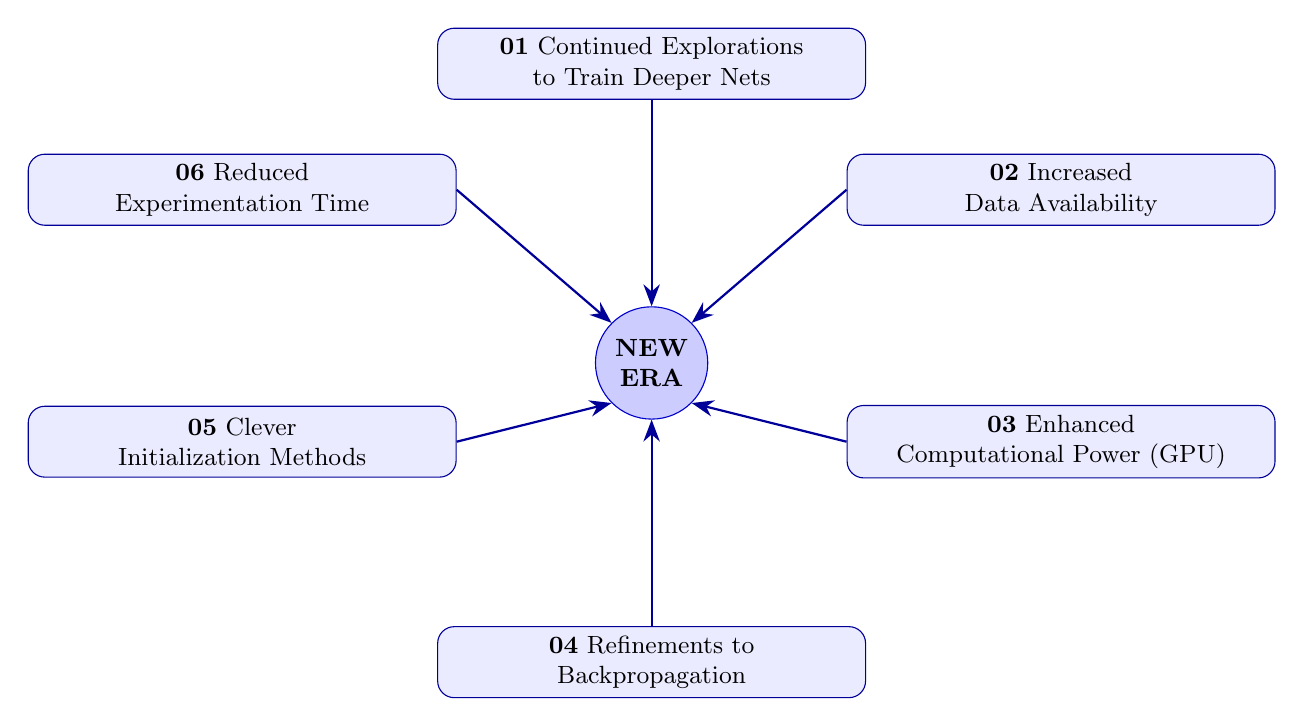
\begin{tikzpicture}[
  factor/.style={
    rectangle, rounded corners=6pt, draw=blue!60!black,
    fill=blue!8!white, text width=5.2cm, align=center,
    minimum height=0.9cm, font=\small
  },
  arrow/.style={-{Stealth[scale=1.2]}, thick, blue!60!black},
  label/.style={font=\bfseries\small, blue!80!black}
]

% Central node
\node[circle, draw=blue!80!black, fill=blue!20!white,
      minimum size=1.4cm, font=\bfseries\small, align=center]
  (center) at (0,0) {NEW\\ERA};

% Six factor nodes placed around the center
\node[factor] (f1) at (0, 3.8)
  {\textbf{01} Continued Explorations\\to Train Deeper Nets};
\node[factor] (f2) at (5.2, 2.2)
  {\textbf{02} Increased\\Data Availability};
\node[factor] (f3) at (5.2, -1.0)
  {\textbf{03} Enhanced\\Computational Power (GPU)};
\node[factor] (f4) at (0, -3.8)
  {\textbf{04} Refinements to\\Backpropagation};
\node[factor] (f5) at (-5.2, -1.0)
  {\textbf{05} Clever\\Initialization Methods};
\node[factor] (f6) at (-5.2, 2.2)
  {\textbf{06} Reduced\\Experimentation Time};

% Arrows pointing inward
\draw[arrow] (f1.south)  -- (center.north);
\draw[arrow] (f2.west)   -- (center.north east);
\draw[arrow] (f3.west)   -- (center.south east);
\draw[arrow] (f4.north)  -- (center.south);
\draw[arrow] (f5.east)   -- (center.south west);
\draw[arrow] (f6.east)   -- (center.north west);

\end{tikzpicture}
\caption{The six converging factors that enabled the deep learning
resurgence (slide V02, 00:22:00).  No single factor sufficed; all six
had to converge.}
\label{fig:six_factors}
\end{figure}

\begin{remark}
\label{rem:not_single_breakthrough}
Prof.\ Prasanna emphasised that the deep learning revolution was
\emph{not} the result of a single new algorithm.  The backpropagation
algorithm itself was not replaced; rather, external conditions
(data and compute) improved while targeted modifications to the
algorithm (weight initialisation and activation functions) addressed
the root cause of training failure.
\end{remark}

% -----------------------------------------------------------
% Table: Timeline of Neural Network Development
% -----------------------------------------------------------
\begin{table}[htbp]
\centering
\caption{Timeline of key milestones in neural network and deep learning
         history as discussed in the lecture.}
\label{tab:timeline}
\begin{tabular}{@{}lll@{}}
\toprule
\textbf{Period} & \textbf{Milestone} & \textbf{Significance} \\
\midrule
1950s--60s & Perceptron model proposed
           & First learnable neuron model \\
1986       & Backpropagation re-popularised
           & Enabled MLP training (2nd breakthrough) \\
Late 1980s & MLP with hidden layers demonstrated
           & Universal approximation capability shown \\
Early 1990s & ``AI hype'' era (neuro-fuzzy, etc.)
            & Performance only matched classical methods \\
Late 1990s & AI winter begins
           & Interest and funding declined \\
$\sim$2000 & Data digitisation explosion
           & Large datasets finally available \\
$\sim$2000 & GPU computing emerges
           & Parallel computation enables larger models \\
2006       & Hinton et al.\ greedy pre-training
           & First practical training of deep nets \\
2006--now  & Deep learning era
           & Continuous performance improvements \\
\bottomrule
\end{tabular}
\end{table}

% ===========================================================
\section{The Vanishing and Exploding Gradient Problem}
\label{sec:vgp}
% ===========================================================

\subsection{The Core Obstacle}
\label{subsec:core_obstacle}

The central problem that prevented deep network training for over a
decade is illustrated in \cref{fig:iceberg}, which reconstructs the
``iceberg diagram'' from lecture slide V03 (timestamp 00:37:35).

% -----------------------------------------------------------
% TikZ Diagram 2: Iceberg diagram (V03)
% -----------------------------------------------------------
\begin{figure}[htbp]
\centering
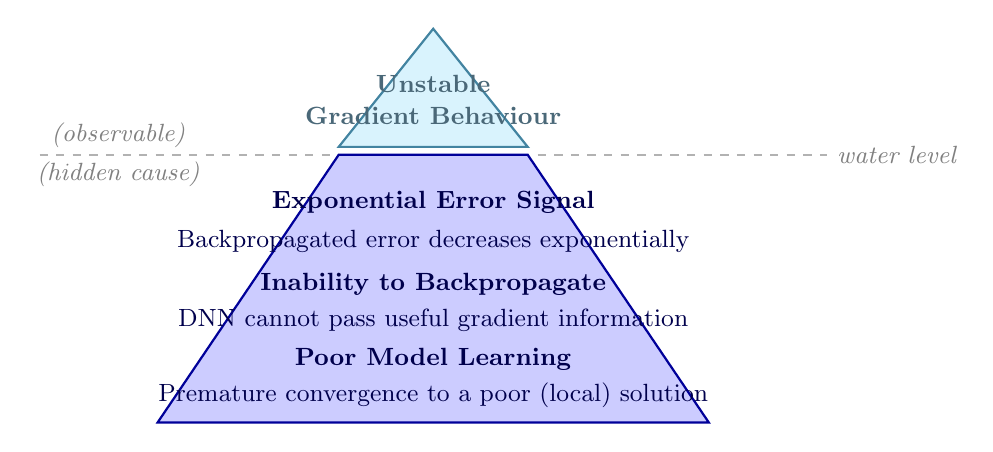
\begin{tikzpicture}[
  visible/.style={fill=cyan!15!white, draw=cyan!60!black, thick},
  hidden/.style={fill=blue!20!white, draw=blue!60!black, thick},
  label_vis/.style={font=\small\bfseries, text=cyan!40!black},
  label_hid/.style={font=\small, text=blue!30!black},
  waterline/.style={dashed, thick, gray!60}
]

% Iceberg tip (visible above water)
\fill[visible]
  (-1.2, 3.5) -- (0, 5.0) -- (1.2, 3.5) -- cycle;
\node[label_vis] at (0, 4.3) {Unstable};
\node[label_vis] at (0, 3.9) {Gradient Behaviour};

% Water line
\draw[waterline] (-5, 3.4) -- (5, 3.4)
  node[right, font=\small\itshape, gray] {water level};
\node[font=\small\itshape, gray] at (-4, 3.65) {(observable)};
\node[font=\small\itshape, gray] at (-4, 3.15) {(hidden cause)};

% Iceberg body (hidden below water)
\fill[hidden]
  (-1.2, 3.4) -- (-3.5, 0.0) -- (3.5, 0.0) -- (1.2, 3.4) -- cycle;

% Labels inside iceberg body
\node[label_hid, align=center] at (0, 2.8)
  {\textbf{Exponential Error Signal}};
\node[label_hid, align=center] at (0, 2.3)
  {Backpropagated error decreases exponentially};
\node[label_hid, align=center] at (0, 1.75)
  {\textbf{Inability to Backpropagate}};
\node[label_hid, align=center] at (0, 1.3)
  {DNN cannot pass useful gradient information};
\node[label_hid, align=center] at (0, 0.8)
  {\textbf{Poor Model Learning}};
\node[label_hid, align=center] at (0, 0.35)
  {Premature convergence to a poor (local) solution};

\end{tikzpicture}
\caption{Iceberg diagram of the VGP/EGP (slide V03, 00:37:35).  The
visible tip -- unstable training behaviour -- is the observable
symptom.  The real cause lies below the surface: exponential decay of
the backpropagated error signal.}
\label{fig:iceberg}
\end{figure}

\subsection{Mathematical Derivation}
\label{subsec:math_derivation}

Consider a network with layers indexed $l = 1, \ldots, L$.  At each
layer the pre-activation is $z^{(l)} = W^{(l)} a^{(l-1)}$ and the
activation is $a^{(l)} = f(z^{(l)})$ for some activation function~$f$.
The gradient of the loss with respect to the weight matrix of layer~1
is, by the chain rule (\cref{eq:backprop_chain}):

\begin{align}
  \frac{\partial \Loss}{\partial W^{(1)}}
  &= \frac{\partial \Loss}{\partial a^{(L)}}
     \cdot \prod_{l=2}^{L}
           \underbrace{f'(z^{(l)}) \cdot W^{(l)}}_{\text{one factor per layer}}
     \cdot x,
  \label{eq:chain_product}
\end{align}

where $x$ is the input.  For the logistic sigmoid, from
\cref{eq:sigmoid_deriv_bound}:

\begin{equation}
  f'(z^{(l)}) = \sigmoid'(z^{(l)}) \;\leq\; 0.25
  \quad \text{for all } z^{(l)}.
  \label{eq:sigmoid_max_deriv}
\end{equation}

If the weights are also initialised with magnitudes $|W^{(l)}| \leq 1$,
then each factor in the product of \cref{eq:chain_product} satisfies:

\begin{equation}
  \left| f'(z^{(l)}) \cdot W^{(l)} \right| \;\leq\; 0.25,
\end{equation}

so the product over $L-1$ layers is bounded by:

\begin{equation}
  \left| \prod_{l=2}^{L} f'(z^{(l)}) \cdot W^{(l)} \right|
  \;\leq\; (0.25)^{L-1}
  = 4^{-(L-1)}.
  \label{eq:exponential_decay}
\end{equation}

\Cref{eq:exponential_decay} shows that the gradient decays
exponentially in the depth $L$.  For a network with only five layers:
$4^{-4} = 1/256 \approx 0.004$ -- less than half a percent of the
original signal.

\begin{example}[title=Layer-by-Layer Gradient Decay]
\label{ex:gradient_decay}
Suppose every sigmoid derivative equals its maximum of $0.25$:
\begin{center}
\begin{tabular}{@{}lll@{}}
\toprule
\textbf{Layer} & \textbf{Gradient factor} & \textbf{Cumulative gradient} \\
\midrule
$L$ (output)   & 1.000 & 1.0000 \\
$L-1$          & $\times\;0.25$ & 0.2500 \\
$L-2$          & $\times\;0.25$ & 0.0625 \\
$L-3$          & $\times\;0.25$ & 0.0156 \\
$L-4$          & $\times\;0.25$ & 0.0039 \\
Layer 1 (input)& $\times\;0.25$ & $\approx 0.001$ \\
\bottomrule
\end{tabular}
\end{center}
By layer 1, the gradient is roughly 1000 times smaller than at the
output.  Weights in the early layers receive no meaningful update
signal.
\end{example}

\subsection{Numerical Walkthrough: Four-Layer Network}
\label{subsec:four_layer}

Dr.\ Saumya demonstrated the VGP with a minimal four-layer network
(one neuron per layer, sigmoid activations, all weights initialised to
$w = 0.5$, biases set to zero, single input $x_1 = 1$, target $y = 0$,
mean-squared loss).

\subsubsection{Forward Pass}
\label{subsubsec:forward}

The forward pass computes:

\begin{align}
  z^{(l)} &= w^{(l)} \cdot a^{(l-1)}, \qquad a^{(l)} = \sigmoid(z^{(l)}),
  \label{eq:forward_pass}
\end{align}

with $a^{(0)} = x_1 = 1$.  The numerical values are:

\begin{align}
  z_1 &= 0.5 \cdot 1 = 0.5, \quad a_1 = \sigmoid(0.5) \approx 0.6225, \notag\\
  z_2 &= 0.5 \cdot 0.6225 \approx 0.3113, \quad a_2 \approx 0.5771, \notag\\
  z_3 &= 0.5 \cdot 0.5771 \approx 0.2885, \quad a_3 \approx 0.5716, \notag\\
  z_4 &= 0.5 \cdot 0.5716 \approx 0.2858, \quad
        \hat{y} = a_4 \approx 0.5709. \label{eq:forward_values}
\end{align}

The loss (with the $\frac{1}{2}$ convenience factor):

\begin{equation}
  \Loss = \frac{1}{2}(\hat{y} - y)^2
        = \frac{1}{2}(0.5709 - 0)^2 \approx 0.1629.
  \label{eq:loss_value}
\end{equation}

\subsubsection{Backward Pass}
\label{subsubsec:backward}

Applying the chain rule from the output backwards:

\begin{align}
  \frac{\partial \Loss}{\partial \hat{y}}
  &= \hat{y} - y = 0.5709, \label{eq:dl_dyhat}\\[6pt]
  \frac{\partial \Loss}{\partial w_4}
  &= \frac{\partial \Loss}{\partial a_4} \cdot \sigmoid'(z_4) \cdot a_3
   \approx 0.5709 \times 0.2450 \times 0.5716
   \approx 0.0799, \label{eq:grad_w4}\\[6pt]
  \frac{\partial \Loss}{\partial w_3}
  &= \frac{\partial \Loss}{\partial w_4\text{-path}} \cdot w_4 \cdot
     \sigmoid'(z_3) \cdot a_2 \approx 0.0300, \label{eq:grad_w3}\\[6pt]
  \frac{\partial \Loss}{\partial w_2}
  &\approx 0.0110, \label{eq:grad_w2}\\[6pt]
  \frac{\partial \Loss}{\partial w_1}
  &\approx 0.0040. \label{eq:grad_w1}
\end{align}

\begin{keyinsight}
The gradient at layer~4 is $\approx 0.0799$.  By the time it reaches
layer~1, it has shrunk to $\approx 0.004$ -- \textbf{about 30 times
smaller}.  With a typical learning rate of $\eta = 0.01$, the weight
update at layer~1 is roughly $\Delta w_1 \approx 4 \times 10^{-5}$,
which is virtually zero.  The early layers \emph{do not learn}.
\end{keyinsight}

% ===========================================================
\section{Detailed Analysis of Sigmoid Saturation}
\label{sec:sigmoid}
% ===========================================================

\subsection{Why Sigmoid Saturates}
\label{subsec:sigmoid_saturation}

The logistic sigmoid function and its derivative are:

\begin{align}
  \sigmoid(z) &= \frac{1}{1 + e^{-z}}, \label{eq:sigmoid_def}\\[6pt]
  \sigmoid'(z) &= \sigmoid(z)\bigl(1 - \sigmoid(z)\bigr). \label{eq:sigmoid_prime}
\end{align}

For large $|z|$, $\sigmoid(z) \to 1$ or $\sigmoid(z) \to 0$.  In
either limit $\sigmoid'(z) \to 0$ because:

\begin{itemize}
  \item If $z \gg 0$: $\sigmoid(z) \approx 1$, so $\sigmoid'(z) \approx 1 \cdot (1-1) = 0$.
  \item If $z \ll 0$: $\sigmoid(z) \approx 0$, so $\sigmoid'(z) \approx 0 \cdot (1-0) = 0$.
\end{itemize}

The derivative is non-zero only in a narrow bell-shaped region around
$z = 0$, with maximum value $0.25$ attained at $z = 0$.  In deep
networks, the pre-activations $z^{(l)}$ frequently escape this narrow
range, driving the sigmoid into its flat regions and killing the
gradient.

\begin{remark}
\label{rem:tanh}
The hyperbolic tangent $\tanh(z) = 2\sigmoid(2z) - 1$ has the same
qualitative saturation behaviour.  Its derivative is bounded by~1
(at $z=0$) and also decays to zero for large $|z|$, so it does not
fundamentally solve the VGP.
\end{remark}

\subsection{Propagation Through Nested Sigmoids}
\label{subsec:nested_sigmoid}

In a deep sigmoid network, successive activations become increasingly
similar (saturate towards $0.5$ for zero-mean inputs).  As shown in
the forward-pass values of \cref{eq:forward_values}, the outputs
$a_1 \approx 0.622$, $a_2 \approx 0.577$, $a_3 \approx 0.572$,
$a_4 \approx 0.571$ differ by less and less -- the network enters the
flat region of the sigmoid, making the derivative contributions
near-zero.  This is the regime where the VGP is most severe.

\begin{warningbox}
In a deep network with sigmoid activations, even without extremely large
or small weights, the \emph{forward activations themselves saturate}.
This is because each sigmoid of a sigmoid of a sigmoid converges to a
fixed point.  The saturation is self-reinforcing: a saturated forward
activation produces a near-zero derivative in the backward pass,
which in turn prevents the early-layer weights from learning the
representations needed to un-saturate those activations.
\end{warningbox}

% -----------------------------------------------------------
% Algorithm: Backpropagation showing gradient decay
% -----------------------------------------------------------
\begin{algorithm}[htbp]
\caption{Backpropagation in a Deep Sigmoid Network (gradient trace)}
\label{alg:backprop_trace}
\SetAlgoLined
\KwIn{Network with $L$ sigmoid layers, weights $\{w^{(l)}\}$,
      input $x$, target $y$}
\KwOut{Gradients $\{\partial\Loss/\partial w^{(l)}\}$,
       showing exponential decay towards layer~1}

\tcp{--- Forward pass ---}
$a^{(0)} \leftarrow x$\;
\For{$l = 1$ \KwTo $L$}{
  $z^{(l)} \leftarrow W^{(l)} a^{(l-1)} + b^{(l)}$\;
  $a^{(l)} \leftarrow \sigmoid(z^{(l)})$\;
}
$\hat{y} \leftarrow a^{(L)}$\;
$\Loss \leftarrow \frac{1}{2}(\hat{y} - y)^2$\;

\tcp{--- Backward pass ---}
$\delta^{(L)} \leftarrow \hat{y} - y$ \tcp*{output gradient}
\For{$l = L$ \KwTo $1$}{
  $\displaystyle
  g^{(l)} \leftarrow \frac{\partial\Loss}{\partial w^{(l)}}
         = \delta^{(l)} \cdot \sigmoid'(z^{(l)}) \cdot a^{(l-1)}$\;
  \tcp{Propagate: each step multiplies by $\sigmoid'(\cdot) \leq 0.25$}
  $\delta^{(l-1)} \leftarrow \delta^{(l)} \cdot \sigmoid'(z^{(l)}) \cdot w^{(l)}$\;
  \texttt{// Note: } $|\delta^{(l-1)}| \leq 0.25 \cdot |\delta^{(l)}|$
  \texttt{ -- exponential decay!}\;
}
\Return $\{g^{(l)}\}_{l=1}^{L}$\;
\end{algorithm}

\subsection{Gradient Magnitude Table}
\label{subsec:gradient_table}

\Cref{tab:gradient_magnitudes} summarises the gradient magnitudes at
each layer in the four-layer demonstration.

\begin{table}[htbp]
\centering
\caption{Gradient magnitudes during backpropagation in the four-layer
         sigmoid network (from the lecture demonstration).  The gradient
         at layer~1 is approximately 30$\times$ smaller than at
         layer~4.}
\label{tab:gradient_magnitudes}
\begin{tabular}{@{}cccc@{}}
\toprule
\textbf{Layer} & \textbf{Activation $a^{(l)}$}
               & \textbf{Sigmoid derivative $\sigmoid'(z^{(l)})$}
               & \textbf{$\|\partial\Loss/\partial w^{(l)}\|$} \\
\midrule
4 (output) & 0.5709 & 0.2450 & 0.0799 \\
3          & 0.5716 & 0.2449 & 0.0300 \\
2          & 0.5771 & 0.2444 & 0.0110 \\
1 (early)  & 0.6225 & 0.2350 & 0.0040 \\
\bottomrule
\end{tabular}
\end{table}

% ===========================================================
\section{Solutions to the Vanishing Gradient Problem}
\label{sec:solutions}
% ===========================================================

Once the root cause was understood, researchers developed a three-step
solution framework, illustrated in \cref{fig:three_step_solution}
(reconstructed from lecture slide V05, timestamp 00:47:00).

% -----------------------------------------------------------
% TikZ Diagram 3: Three-step solution (V05)
% -----------------------------------------------------------
\begin{figure}[htbp]
\centering
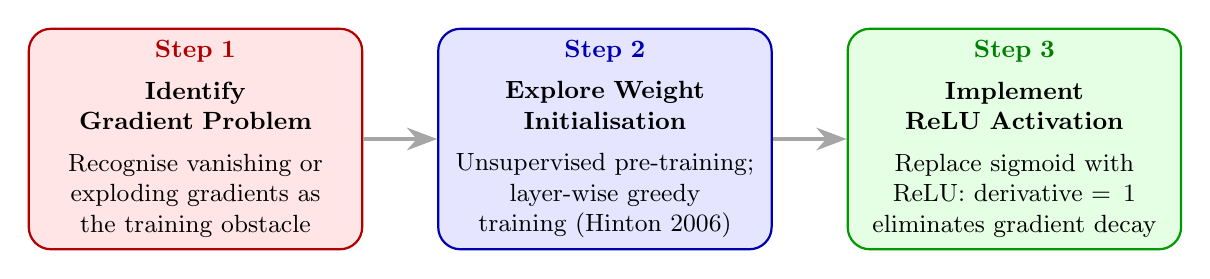
\begin{tikzpicture}[
  box/.style={
    rectangle, rounded corners=8pt, draw, thick,
    text width=4.0cm, align=center, minimum height=2.8cm,
    font=\small
  },
  step1/.style={box, fill=red!10!white,   draw=red!70!black},
  step2/.style={box, fill=blue!10!white,  draw=blue!70!black},
  step3/.style={box, fill=green!10!white, draw=green!60!black},
  arr/.style={-{Stealth[scale=1.3]}, very thick, gray!70}
]

\node[step1] (s1) at (0,0) {
  \textcolor{red!70!black}{\textbf{Step 1}}\\[4pt]
  \textbf{Identify}\\
  \textbf{Gradient Problem}\\[4pt]
  Recognise vanishing or\\exploding gradients as\\the training obstacle
};

\node[step2] (s2) at (5.2,0) {
  \textcolor{blue!70!black}{\textbf{Step 2}}\\[4pt]
  \textbf{Explore Weight}\\
  \textbf{Initialisation}\\[4pt]
  Unsupervised pre-training;\\layer-wise greedy\\training (Hinton 2006)
};

\node[step3] (s3) at (10.4,0) {
  \textcolor{green!50!black}{\textbf{Step 3}}\\[4pt]
  \textbf{Implement}\\
  \textbf{ReLU Activation}\\[4pt]
  Replace sigmoid with\\ReLU: derivative~$=1$\\eliminates gradient decay
};

\draw[arr] (s1.east) -- (s2.west);
\draw[arr] (s2.east) -- (s3.west);

\end{tikzpicture}
\caption{Three-step solution framework for VGP/EGP (slide V05,
         00:47:00).}
\label{fig:three_step_solution}
\end{figure}

\subsection{Solution 1 -- Weight Initialisation}
\label{subsec:weight_init}

The standard approach of \emph{random} initialisation starts the
network in a region of parameter space that may be far from anything
useful.  For deep networks, this is particularly harmful because even a
moderately poor initialisation places activations in the saturated
regions of sigmoid.

\subsubsection{Hinton's Greedy Layer-Wise Pre-Training (2006)}
\label{subsubsec:greedy_pretrain}

The breakthrough method proposed by Hinton, Osindero, and Teh (2006)
used \emph{unsupervised greedy pre-training} in a layer-wise fashion:

\begin{enumerate}
  \item Train the first layer as a Restricted Boltzmann Machine (RBM)
        or a simple autoencoder: learn weights $W^{(1)}$ that
        reconstruct the input from the first hidden representation.
        Minimise reconstruction error:
        \begin{equation}
          \Loss_1 = \bigl\| x - \hat{x}^{(1)} \bigr\|^2.
          \label{eq:recon_loss_1}
        \end{equation}
  \item Freeze $W^{(1)}$.  Use the learned representation $h^{(1)}$
        as the new ``input'' and train the second layer similarly:
        \begin{equation}
          \Loss_2 = \bigl\| h^{(1)} - \hat{h}^{(1)} \bigr\|^2.
          \label{eq:recon_loss_2}
        \end{equation}
  \item Repeat layer by layer up to depth~$L$.
  \item Use the pre-trained weights as the \emph{initialisation} for
        supervised fine-tuning via standard backpropagation.
\end{enumerate}

\begin{keyinsight}
Greedy pre-training solves the VGP indirectly: because each layer's
weights are already initialised to encode meaningful features of the
data (rather than random noise), the forward activations do not
immediately saturate, and backpropagation can usefully propagate
gradients all the way to the first layer.
\end{keyinsight}

\subsubsection{Modern Initialisation Methods}
\label{subsubsec:modern_init}

After 2010, it was found that carefully chosen random initialisations
could also avoid saturation at the start of training.  The two most
widely used are:

\begin{itemize}
  \item \textbf{Xavier / Glorot initialisation} (Glorot \&\ Bengio 2010):
        \begin{equation}
          W^{(l)} \sim \mathcal{U}\!\left(
            -\sqrt{\frac{6}{n_{\mathrm{in}}+n_{\mathrm{out}}}},\;
            +\sqrt{\frac{6}{n_{\mathrm{in}}+n_{\mathrm{out}}}}
          \right),
          \label{eq:xavier_init}
        \end{equation}
        where $n_{\mathrm{in}}$ and $n_{\mathrm{out}}$ are the number
        of input and output neurons of layer~$l$.  Designed to keep
        activation variances approximately constant across layers for
        sigmoid and tanh networks.

  \item \textbf{He initialisation} (He et al.\ 2015):
        \begin{equation}
          W^{(l)} \sim \mathcal{N}\!\left(
            0,\; \frac{2}{n_{\mathrm{in}}}
          \right),
          \label{eq:he_init}
        \end{equation}
        designed for ReLU activations.

  \item \textbf{Batch Normalisation} (Ioffe \&\ Szegedy 2015):
        normalises layer inputs to have zero mean and unit variance
        during each mini-batch, re-centering activations into the
        non-saturating region of sigmoid/tanh.
\end{itemize}

\subsection{Solution 2 -- ReLU Activation Function}
\label{subsec:relu}

The second major solution is to replace the sigmoid activation with
the \emph{Rectified Linear Unit}:

\begin{equation}
  \relu(z) = \max(0, z),
  \label{eq:relu_def}
\end{equation}

whose derivative is:

\begin{equation}
  \relu'(z) =
  \begin{cases}
    1 & \text{if } z > 0, \\
    0 & \text{if } z \leq 0.
  \end{cases}
  \label{eq:relu_deriv}
\end{equation}

When $z > 0$, the gradient is exactly~1 and does not shrink through
any number of layers.  This means:

\begin{equation}
  \prod_{l=2}^{L} \relu'(z^{(l)}) \in \{0, 1\},
  \quad\text{no exponential decay for active neurons.}
  \label{eq:relu_product}
\end{equation}

\begin{example}[title=ReLU Gradient Does Not Vanish]
\label{ex:relu_gradient}
With ReLU activations (and all pre-activations $z^{(l)} > 0$), the
gradient chain is:
\begin{center}
\begin{tabular}{@{}lll@{}}
\toprule
\textbf{Layer} & \textbf{ReLU derivative} & \textbf{Cumulative gradient} \\
\midrule
$L$   & 1 & 1.0 \\
$L-1$ & 1 & 1.0 \\
$L-2$ & 1 & 1.0 \\
$L-3$ & 1 & 1.0 \\
Layer 1 & 1 & 1.0 \\
\bottomrule
\end{tabular}
\end{center}
The gradient magnitude is preserved all the way to the first layer.
Compare with the sigmoid case in \cref{ex:gradient_decay}.
\end{example}

\subsubsection{ReLU Non-Linearity and the Dead Neuron Problem}
\label{subsubsec:dead_neuron}

A student raised an important question during the lecture: \emph{``Why
is ReLU preferred over tanh for the vanishing gradient, even though
ReLU can cause dead neurons?''}

ReLU is indeed non-linear (the ``kink'' at $z = 0$ breaks linearity),
which is necessary for deep networks to model complex functions.  For
$z > 0$ it is linear, making it easy to optimise and very fast to
compute.

However, the \emph{dying ReLU} problem arises when a neuron's
pre-activation $z^{(l)} \leq 0$ for all training samples, causing its
gradient to be identically zero and its weights to never update.
Variants of ReLU were proposed to address this:

\begin{description}
  \item[Leaky ReLU:] $f(z) = \max(\alpha z, z)$ for small
        $\alpha > 0$ (e.g.\ $\alpha = 0.01$), allowing a small negative
        gradient for $z < 0$.
  \item[ELU (Exponential Linear Unit):] $f(z) = z$ for $z \geq 0$,
        $\alpha(e^z - 1)$ for $z < 0$.
  \item[GELU (Gaussian Error Linear Unit):] $f(z) = z \cdot
        \Phi(z)$, used in Transformers.
\end{description}

\subsubsection{Sigmoid vs.\ ReLU: Full Comparison}
\label{subsubsec:sig_relu_comparison}

\Cref{tab:sig_vs_relu} gives the full comparison as presented in the
lecture visual extraction.

\begin{table}[htbp]
\centering
\caption{Comparison of sigmoid and ReLU activation functions.}
\label{tab:sig_vs_relu}
\begin{tabular}{@{}lll@{}}
\toprule
\textbf{Property}
  & \textbf{Sigmoid $\sigma(x)$}
  & \textbf{ReLU $\max(0,x)$} \\
\midrule
Output range    & $(0,\,1)$   & $[0,\,+\infty)$ \\
Derivative range & $(0,\,0.25]$ & $\{0,\,1\}$ \\
Vanishing gradient & \textbf{Yes} -- saturates at extremes
                   & \textbf{No} -- constant~1 for $x>0$ \\
Computational cost & Expensive ($e^{-x}$) & Very fast ($\max$) \\
Dying neurons      & No & \textbf{Yes} (for $x \leq 0$) \\
Biological plausibility & Higher & Lower \\
Typical use case  & Output layer (binary classification)
                  & Hidden layers (default choice) \\
\bottomrule
\end{tabular}
\end{table}

% ===========================================================
\section{Addressing VGP/EGP: Integrated View}
\label{sec:integrated_view}
% ===========================================================

\subsection{Why Both Solutions are Needed}
\label{subsec:both_needed}

ReLU alone does not fully eliminate the VGP.  Dead neurons create
regions of zero gradient that are structurally similar to sigmoid
saturation.  Likewise, good initialisation alone does not help if the
activation function accumulates saturation as training progresses.

The combination of \emph{better initialisation} and \emph{ReLU
activations} together proved sufficient to train the deep networks of
the 2006--2012 era.  Subsequent advances -- batch normalisation,
residual connections, and attention mechanisms -- further generalised
these principles.

\subsection{Layer-Wise Training: Modular Construction Analogy}
\label{subsec:layerwise}

Prof.\ Prasanna used an instructive analogy: layer-wise pre-training
is like modular construction in civil engineering.  Each module (layer)
is first built and tested in isolation, then assembled into the
complete structure.  In neural network terms:

\begin{itemize}
  \item Train (input $\to$ layer 1 $\to$ reconstruction of input).
  \item Freeze layer 1.  Train (layer 1 output $\to$ layer 2 $\to$
        reconstruction of layer 1 output).
  \item Repeat until all layers are pre-trained.
  \item Fine-tune the whole network end-to-end with backpropagation,
        using the pre-trained weights as a starting point.
\end{itemize}

The key insight is that the gradient only needs to travel through
\emph{one or two layers} during pre-training, so it never has a chance
to vanish.

\begin{keyinsight}
The backpropagation algorithm itself was \emph{not} discarded in the
deep learning revolution.  The community diagnosed exactly what was
going wrong (vanishing gradients due to sigmoid saturation and poor
initialisation) and applied targeted fixes.  The core algorithm
remained intact.
\end{keyinsight}

\subsection{Modern Perspective}
\label{subsec:modern_perspective}

Today, the dominant solution stack for avoiding VGP/EGP in practice is:

\begin{enumerate}
  \item \textbf{ReLU (or variant) activations} in all hidden layers.
  \item \textbf{He initialisation} for ReLU networks.
  \item \textbf{Batch Normalisation} after linear layers to maintain
        stable activation distributions during training.
  \item \textbf{Residual (skip) connections} (ResNet, 2015): allow
        the gradient to bypass entire blocks, providing ``shortcut''
        paths for the gradient that do not pass through activation
        functions.
\end{enumerate}

The greedy layer-wise pre-training of Hinton~(2006) is now largely of
historical interest, having been superseded by the above stack, but it
was the critical proof-of-concept that made the deep learning era
possible.

% ===========================================================
\section{Summary and Conclusions}
\label{sec:summary}
% ===========================================================

Session~8 covered the pivotal transition from shallow ANNs to deep
networks.  The following table summarises the key conceptual
contributions.

\begin{table}[htbp]
\centering
\caption{Session 8 -- Summary of key topics.}
\label{tab:summary}
\begin{tabular}{@{}p{4.2cm}p{9cm}@{}}
\toprule
\textbf{Topic} & \textbf{Key Message} \\
\midrule
Historical context
  & Deep networks were envisioned in the 1990s but could not be
    trained for $\sim$15 years due to the VGP. \\[4pt]
Six enabling factors
  & The deep learning revival was a convergence of data, compute,
    and algorithmic refinements -- not a single breakthrough. \\[4pt]
Vanishing gradient problem
  & Sigmoid derivatives $\leq 0.25$ cause gradients to shrink as
    $(0.25)^{L-1}$ exponentially with depth, starving early layers
    of training signal. \\[4pt]
Exploding gradient problem
  & Symmetric pathology; arises from floating-point overflow when
    derivatives compound in the forward direction. \\[4pt]
Weight initialisation
  & Hinton's greedy layer-wise unsupervised pre-training (2006)
    provided meaningful starting weights; modern alternatives
    include Xavier and He initialisation. \\[4pt]
ReLU activation
  & $\relu(z) = \max(0,z)$ has derivative~1 for $z>0$, preventing
    gradient decay; also computationally fast. \\[4pt]
Dead neuron problem
  & ReLU gradient is 0 for $z \leq 0$; addressed by Leaky ReLU,
    ELU, and other variants. \\
\bottomrule
\end{tabular}
\end{table}

\subsection{Looking Ahead}
\label{subsec:looking_ahead}

The next session continues the deep learning journey, examining
specific deep architectures (Convolutional Neural Networks, Recurrent
Neural Networks) and their training in detail.  The solutions
introduced here -- ReLU activations and principled weight
initialisation -- underpin all modern deep learning systems and will
appear repeatedly throughout the rest of the course.

\begin{keyinsight}
The deep learning era did not begin because computers got faster or
datasets grew larger in isolation.  It began because a small group of
researchers refused to abandon the field during its winter,
methodically diagnosed the root cause of training failure, and devised
solutions elegant enough to be adopted universally.
\end{keyinsight}

% ===========================================================
% APPENDIX
% ===========================================================
\appendix

\section{Mathematical Derivation: Sigmoid Derivative Upper Bound}
\label{app:sigmoid_bound}

\begin{theorem}
\label{thm:sigmoid_bound}
For the logistic sigmoid $\sigmoid(z) = \frac{1}{1+e^{-z}}$, the
derivative satisfies $\sigmoid'(z) \leq \frac{1}{4}$ for all
$z \in \mathbb{R}$.
\end{theorem}

\begin{proof}
From \cref{eq:sigmoid_prime}, $\sigmoid'(z) = \sigmoid(z)(1-\sigmoid(z))$.
Let $s = \sigmoid(z) \in (0,1)$.  We need to show $s(1-s) \leq 1/4$.
By AM-GM, $s(1-s) \leq \left(\frac{s + (1-s)}{2}\right)^2 = \frac{1}{4}$,
with equality iff $s = 1-s$, i.e.\ $s = 1/2$, i.e.\ $z = 0$.
\end{proof}

\begin{lemma}
\label{lem:product_decay}
For a sigmoid network with $L$ layers and weight magnitudes
$|W^{(l)}| \leq 1$, the gradient satisfies:
\begin{equation}
  \left|\frac{\partial\Loss}{\partial W^{(1)}}\right|
  \;\leq\;
  \left|\frac{\partial\Loss}{\partial a^{(L)}}\right|
  \cdot \left(\frac{1}{4}\right)^{L-1}.
  \label{eq:decay_bound}
\end{equation}
\end{lemma}

\begin{proof}
Follows directly from \cref{eq:chain_product,eq:sigmoid_max_deriv}
and the assumption $|W^{(l)}| \leq 1$.
\end{proof}

\section{ReLU Variants Reference}
\label{app:relu_variants}

\begin{table}[htbp]
\centering
\caption{Summary of ReLU variants mentioned in the lecture.}
\label{tab:relu_variants}
\begin{tabular}{@{}llll@{}}
\toprule
\textbf{Name} & \textbf{Definition} & \textbf{Derivative ($z<0$)}
              & \textbf{Notes} \\
\midrule
ReLU & $\max(0,z)$ & 0 & Standard; may cause dead neurons \\
Leaky ReLU & $\max(\alpha z, z)$ & $\alpha$ & $\alpha \approx 0.01$;
              prevents dead neurons \\
ELU & $z \geq 0$: $z$; $z<0$: $\alpha(e^z-1)$ & $\alpha e^z$ &
      Smooth; negative mean push \\
SELU & Self-normalising ELU & scaled & Auto-normalises activations \\
GELU & $z\,\Phi(z)$ & $\Phi(z) + z\phi(z)$ &
       Used in BERT, GPT \\
\bottomrule
\end{tabular}
\end{table}

\end{document}
